\documentclass[10pt]{article}
\usepackage[spanish]{babel}
\usepackage[a4paper, tmargin=0.75in, lmargin=0.80in, rmargin=0.80in, bmargin=1in]{geometry}
\usepackage{hyperref}
%\usepackage{multicol}
\hypersetup{
    colorlinks=true,
    linkcolor=black,
    filecolor=magenta,      
    urlcolor=blue,
    citecolor=black,
}
%\usepackage[numbers,sort&compress]{natbib} % for a numerical citation list
\usepackage{natbib} % to cite references by surname and year
\usepackage{graphicx}
\usepackage{amsfonts}
\usepackage{amsthm}
\usepackage{amssymb}
\usepackage{lipsum}
\usepackage{amsmath}
\usepackage{tabularx}
\usepackage{pdflscape}
\usepackage{booktabs}
\usepackage{bbm}
\usepackage{listings}
\usepackage{xcolor}

\usepackage[
  backend=biber,
  style=alphabetic,
  citestyle=alphabetic,
  doi=true,
  url=true,
  isbn=false,
  eprint=false,
  maxbibnames=99
]{biblatex}

\addbibresource{referencias.bib}

% Definimos colores estilo "terminal con fondo negro"
\definecolor{backcolour}{rgb}{0.1,0.1,0.1}
\definecolor{codegreen}{rgb}{0,0.8,0}
\definecolor{codegray}{rgb}{0.7,0.7,0.7}
\definecolor{codepurple}{rgb}{0.8,0.6,1}
\definecolor{codewhite}{rgb}{1,1,1}


\lstdefinestyle{mypython}{
    backgroundcolor=\color{backcolour},
    basicstyle=\ttfamily\scriptsize\color{codewhite},
    commentstyle=\color{codegreen},
    keywordstyle=\color{codepurple},
    stringstyle=\color{codegreen},
    numbers=left,
    numberstyle=\tiny\color{codegray},
    breaklines=true,
    breakatwhitespace=false,
    showstringspaces=false,
    tabsize=4
}

\lstset{style=mypython}







\pagestyle{empty}


%%%%%%%%%%%%%%%%%%%%%%%%%%%%%%%%%%%%%%%%%%%%%%%%%%
%%%%%%%%%%%%%%%%%%%%%%%%%%%%%%%%%%%%%%%%%%%%%%%%%%
%%%%%%%%%%%%%%%%%%%%%%%%%%%%%%%%%%%%%%%%%%%%%%%%%%
%%%%%%%%%%%%%%%%%%%%%%%%%%%%%%%%%%%%%%%%%%%%%%%%%%
% ENTER SOME IMPORTANT INFORMATION
%%%%%%%%%%%%%%%%%%%%%%%%%%%%%%%%%%%%%%%%%%%%%%%%%%
%%%%%%%%%%%%%%%%%%%%%%%%%%%%%%%%%%%%%%%%%%%%%%%%%%
%%%%%%%%%%%%%%%%%%%%%%%%%%%%%%%%%%%%%%%%%%%%%%%%%%
%%%%%%%%%%%%%%%%%%%%%%%%%%%%%%%%%%%%%%%%%%%%%%%%%%
\newcommand{\studentname}{Sánchez, Hazel; Hernández, Debany ; Canché, Elías}
\newcommand{\researchcentre}{Maestría en Probabilidad y Estadística}
\newcommand{\institution}{Centro de Investigación en Matemáticas (CIMAT)}
\newcommand{\projecttitle}{Tarea 2}
\newcommand{\supervisor}{Dr. Marco Antonio Aquino López}
%%%%%%%%%%%%%%%%%%%%%%%%%%%%%%%%%%%%%%%%%%%%%%%%%%
%%%%%%%%%%%%%%%%%%%%%%%%%%%%%%%%%%%%%%%%%%%%%%%%%%
%%%%%%%%%%%%%%%%%%%%%%%%%%%%%%%%%%%%%%%%%%%%%%%%%%
%%%%%%%%%%%%%%%%%%%%%%%%%%%%%%%%%%%%%%%%%%%%%%%%%%
%%%%%%%%%%%%%%%%%%%%%%%%%%%%%%%%%%%%%%%%%%%%%%%%%%
%%%%%%%%%%%%%%%%%%%%%%%%%%%%%%%%%%%%%%%%%%%%%%%%%%

\begin{document}

\begin{center}
{\Large{Proyecto 2: Clasificación Supervisada}} \\
\vspace{2mm}
{\Large{Introducción a la Ciencia de Datos}} \\
\end{center}

\vspace{5mm}
\hrule
\vspace{1mm}
\hrule

\vspace{3mm}
\begin{tabular}{ll} 
Integrantes:           	        & {\studentname}   \\ 
Programa Educativo: 	        & {\researchcentre}  \\ 
Institución:                 & {\institution}  \\
Profesor: 	                 & {\supervisor}  \\ 
\end{tabular}

\vspace{3mm}
\hrule
\vspace{1mm}
\hrule

\begin{abstract}

\end{abstract}

\section{Introducción}
En el marketing digital y la gestión de relaciones con el cliente, la capacidad de predecir comportamientos del consumidor es una herramienta importante para las empresas. A diferencia del marketing convencional, el marketing digital permite una interacción directa y personalizada con los consumidores facilitando la promoción de productos y servicios, además de la recolección de datos sobre el comportamiento y las preferencias del público objetivo. En un entorno comercial cada vez más competido, esta capacidad de capturar y analizar información se traduce en ventajas de mercado.\\

La Ciencia de Datos, con técnicas de clasificación supervisada, proporciona herramientas para identificar patrones ocultos, predecir comportamientos futuros y optimizar recursos, también es posible obtener modelos predictivos que identifican clientes con mayor probabilidad de responder positivamente a una campaña, lo cual podría maximizar el retorno de inversión y fortalecer las estrategias de fidelización del cliente.\\

En este trabajo aplicamos diversos métodos de clasificación supervisada sobre la base de datos ``Bank Marketing'', la cual documenta campañas de marketing directo realizadas por un banco portugués entre 2008 y 2013, cuyo objetivo fundamental fue identificar clientes propensos a suscribir depósitos a plazo.\\

Más allá de la implementación técnica, proponemos examinar cómo la naturaleza de los datos influye en el desempeño de cada clasificador. El análisis se estructura en tres fases: una exploración exhaustiva de las variables y sus relaciones, un procesamiento que incluye codificación de variables categóricas y manejo de desbalance de clases (en caso de encontrar), y una evaluación de los métodos mediante métricas múltiples que capturen distintos aspectos del desempeño predictivo.


\section{Exploración inicial de los datos}\label{sec:dataset}

\subsection{\textit{Bank Marketing Dataset}.}

El \textbf{Bank Marketing Dataset} (\texttt{bank-full.csv}) fue desarrollado y publicado por el Instituto de Sistemas e Informática (INESC) de la Universidad de Lisboa, Portugal, como parte de un estudio longitudinal sobre efectividad de campañas de marketing en el sector bancario. Los datos fueron recolectados entre mayo de 2008 y noviembre de 2013 a través de campañas de marketing telefónico realizadas por una institución bancaria portuguesa y contiene información sobre clientes y el resultado de campañas de marketing telefónicas.\\

La estructura general de la base de datos consta de 45,211 observaciones, 16 variables predictoras y 1 variable de respuesta que indica si el cliente aceptó (\texttt{yes}) o no (\texttt{no}) contratar el depósito a plazo. En la tabla [\ref{tab:clasificacion_predictores}] se describen a detalle las variables, mientras que en las tablas [\ref{tab:estadisticas_numericas}] y [\ref{tab:resumen_categoricas}] se muestra un resumen sobre la información de la base de datos respecto a cada variable.\\

\begin{table}[h!]
\centering
\caption{Clasificación de Variables Predictoras del Bank Marketing Dataset}
\label{tab:clasificacion_predictores}
\begin{tabular}{p{1.7cm} p{1.8cm} p{1.2cm} p{9.4cm}}
\toprule
\textbf{Variable} & \textbf{Tipo} & \textbf{Escala} & \textbf{Descripción y Características} \\
\midrule
age & Numérica & Continua & Edad del cliente (17-98 años). Distribución aprox. normal. \\
job & Categórica & Nominal & Ocupación 13 categorías. \\
marital & Categórica & Nominal & Estado civil: 'divorced', 'married', 'single', 'unknown'. \\
education & Categórica & Ordinal & Nivel educativo: 'basic.4y', 'basic.6y', 'basic.9y', 'high.school', 'illiterate', 'professional.course', 'university.degree', 'unknown'. \\
default & Categórica & Binaria & Crédito en mora: 'no', 'yes', 'unknown'. \\
housing & Categórica & Binaria & Préstamo hipotecario: 'no', 'yes', 'unknown'.\\
loan & Categórica & Binaria & Préstamo personal: 'no', 'yes', 'unknown'. \\
contact & Categórica & Nominal & Tipo de contacto: 'cellular', 'telephone'. \\
month & Categórica & Ordinal & Mes último contacto: 'jan' a 'dec'. \\
day\_of\_week & Categórica & Ordinal & Día último contacto: 'mon' a 'fri'. \\
duration & Numérica & Continua & Duración de contacto (segundos). \\
campaign & Numérica & Discreta & Número de contactos en campaña actual. \\
pdays & Numérica & Discreta & Días desde último contacto. \\
previous & Numérica & Discreta & Número de contactos anteriores. \\
poutcome & Categórica & Nominal & Resultado campaña anterior: 'failure', 'nonexistent', 'success'. \\
emp.var.rate & Numérica & Continua & Tasa variación empleo (trimestral). \\
cons.price.idx & Numérica & Continua & Índice precios al consumidor (mensual). \\
cons.conf.idx & Numérica & Continua & Índice confianza del consumidor (mensual).\\
euribor3m & Numérica & Continua & Tasa Euribor 3 meses (diaria). \\
nr.employed & Numérica & Continua & Número de empleados (trimestral). \\
\bottomrule
\end{tabular}
\end{table}

\begin{table}[h!]
\centering
\caption{Estadísticas Descriptivas de Variables Numéricas}
\label{tab:estadisticas_numericas}
\begin{tabular}{lrrrrr}
\hline
\textbf{Variable} & \textbf{Media} & \textbf{Desv. Est.} & \textbf{Mínimo} & \textbf{Máximo} & \textbf{Asimetría} \\
\hline
age & 40.94 & 10.62 & 17 & 98 & 0.69 \\
duration & 258.28 & 259.28 & 0 & 4918 & 4.97 \\
campaign & 2.76 & 3.10 & 1 & 63 & 9.13 \\
pdays & 962.48 & 186.91 & 0 & 999 & -4.50 \\
previous & 0.17 & 0.49 & 0 & 7 & 6.57 \\
emp.var.rate & 0.08 & 1.57 & -3.4 & 1.4 & -0.79 \\
cons.price.idx & 93.58 & 0.58 & 92.20 & 94.77 & -0.37 \\
cons.conf.idx & -40.50 & 4.63 & -50.8 & -26.9 & 0.57 \\
euribor3m & 3.62 & 1.73 & 0.63 & 5.04 & -0.73 \\
nr.employed & 5167.03 & 72.25 & 4964 & 5228 & -0.53 \\
\hline
\end{tabular}
\end{table}



\begin{table}[h!]
\centering
\caption{Resumen Estadístico de Variables Categóricas}
\label{tab:resumen_categoricas}
\begin{tabular}{p{1.7cm} p{1cm} p{2.3cm} p{9cm}}
\toprule
\textbf{Variable} & \textbf{N°Cat.} & \textbf{Moda} & \textbf{Distribución y Observaciones} \\
\midrule
job & 12 & admin. (22.9\%) & 
\begin{minipage}{7cm}
admin. (22.9\%), blue-collar (21.6\%), technician (15.7\%), services (11.5\%), management (10.9\%), retired (4.0\%), entrepreneur (3.6\%), self-employed (3.5\%), housemaid (2.8\%), unemployed (2.1\%), student (1.0\%), unknown (0.3\%)
\end{minipage} \\
\midrule
marital & 4 & married (60.2\%) & 
\begin{minipage}{7cm}
married (60.2\%), single (28.5\%), divorced (11.1\%), unknown (0.2\%)
\end{minipage} \\
\midrule
education & 8 & university.degree (22.8\%) & 
\begin{minipage}{7cm}
university.degree (22.8\%), high.school (20.7\%), basic.9y (14.6\%), professional.course (14.2\%), basic.4y (10.8\%), basic.6y (9.8\%), unknown (5.0\%), illiterate (0.2\%)
\end{minipage} \\
\midrule
default & 3 & no (98.9\%) & 
\begin{minipage}{7cm}
no (98.9\%), unknown (0.9\%), yes (0.2\%)\\
\textbf{Alto desbalance} - Considerar eliminar o agrupar
\end{minipage} \\
\midrule
housing & 3 & yes (55.6\%) & 
\begin{minipage}{7cm}
yes (55.6\%), no (44.4\%), unknown (0.1\%)\\
\end{minipage} \\
\midrule
loan & 3 & no (82.0\%) & 
\begin{minipage}{7cm}
no (82.0\%), yes (18.0\%), unknown (0.1\%)
\end{minipage} \\
\midrule
contact & 2 & cellular (64.4\%) & 
\begin{minipage}{7cm}
cellular (64.4\%), telephone (35.6\%)\\
\end{minipage} \\
\midrule
month & 12 & may (30.5\%) & 
\begin{minipage}{7cm}
may (30.5\%), jul (13.7\%), aug (13.1\%), jun (12.1\%), nov (9.6\%), apr (5.8\%), oct (4.9\%), mar (4.3\%), sep (3.2\%), dec (1.3\%), jan (0.9\%), feb (0.5\%)\\
\textbf{Estacionalidad} - Picos en primavera/verano
\end{minipage} \\
\midrule
day\_of\_week & 5 & thu (22.8\%) & 
\begin{minipage}{7cm}
thu (22.8\%), wed (22.3\%), tue (21.3\%), mon (20.7\%), fri (12.9\%)\\
\end{minipage} \\
\midrule
poutcome & 3 & nonexistent (85.3\%) & 
\begin{minipage}{7cm}
nonexistent (85.3\%), failure (14.5\%), success (0.2\%)\\
\textbf{Desbalance extremo} - Solo 0.2\% de éxitos previos
\end{minipage} \\
\bottomrule
\end{tabular}
\end{table}

El análisis exploratorio reveló problemas en las variables categóricas que requieren tratamiento específico durante el preprocesamiento. Se identificó alto desbalance en varias variables: la variable default presenta una concentración extrema del 98.9\% en la categoría "no", lo que sugiere considerar su eliminación del modelo; poutcome muestra una distribución problemática con 85.3\% en "nonexistent" y solo 0.2\% en "success", recomendándose agrupar categorías; y loan presenta un desbalance moderado con 82.0\% en "no", donde técnicas de ponderación podrían mejorar el modelado. Adicionalmente, el problema de valores desconocidos afecta significativamente a education (5.0\% unknown), donde la imputación por moda resulta apropiada; job (0.3\% unknown) podría resolverse mediante eliminación o imputación simple; y default (0.9\% unknown) donde considerar "unknown" como categoría separada preservaría información potencialmente valiosa. Estos hallazgos destacan la necesidad de estrategias de preprocesamiento diferenciadas para garantizar la calidad predictiva de los modelos.


Respecto a los \textbf{valores faltantes}, no se detectaron celdas con \texttt{NaN}. Sin embargo, algunas variables categóricas presentan la categoría \texttt{unknown}, la cual representa información faltante implícita (especialmente en \texttt{job}, \texttt{marital}, \texttt{education} y \texttt{contact}). Este aspecto deberá considerarse en la fase de preprocesamiento, ya sea tratándola como una categoría válida o mediante imputación o eliminación. En cuanto a los \textbf{duplicados}, no se encontraron registros repetidos.\\ 

Finalmente, la \textbf{variable de respuesta \texttt{y}} se encuentra desbalanceada: aproximadamente el \textbf{88.3\% de los registros corresponden a ``no''} y solo el \textbf{11.7\% a ``yes''}. Este desbalance es relevante, pues implica que las técnicas de modelado deberán considerar métodos para equilibrar la predicción, como métricas apropiadas (F1, recall) o técnicas de balanceo de clases. 



\newpage
\section{Preprocesamiento}
El preprocesamiento tiene como finalidad transformar la base de datos \textbf{Bank Marketing} (\texttt{bank-full.csv} en una matriz de diseño adecuado para el modelado supervisado. En particular, buscamos, 
\begin{itemize}
    \item[i)] representar de forma numérica las variables categóricas preservando su información, 
    \item[ii)] homogenizar la escala de las variables numéricas para algoritmos sensibles a la magnitud, 
    \item[iii)] separar correctamente predictores $X$ y respuesta $y$ evitando fugas de información. 
\end{itemize}

\subsection*{Preparación y limpieza}
Como paso inicial, se normalizó el formato de las variables categóricas (\textit{trimming} de espacios y conversión a minúsculas) para evitar duplicidades por diferencias de capitalización o espacios. La variable de respuesta \(\texttt{y}\) se codificó como binaria $(0=\texttt{no}$, $1=\texttt{yes}$).

\subsection*{Codificación de variables categóricas}
Las variables cualitativas (\texttt{job}, \texttt{marital}, \texttt{education}, \texttt{contact}, \texttt{month}, \texttt{poutcome}, entre otras) se trataron como nominales y se transformaron mediante \textbf{One-Hot Encoding} (creación de indicadores binarios por categoría). Esta estrategia nos ayuda a:  
\begin{itemize}
    \item Evitar imponer un orden arbitrario sobre categorías no ordinales.
    \item Permite a los modelos lineales asignar efectos específicos por categoría.
    \item Facilita la interpretación al nivel de categoría (coeficientes por indicador).
\end{itemize}

Para garantizar una matriz de diseño de \emph{rango completo}, se utilizó la opción \texttt{drop\_first=True}, eliminando una categoría de referencia por variable (conocido como \emph{dummy variable trap}). En términos prácticos, si \texttt{marital} tiene categorías \{\texttt{married}, \texttt{single}, \texttt{divorced}\}, tras la codificación con referencia en \texttt{married} se generan dos columnas (\texttt{marital\_single}, \texttt{marital\_divorced}); un registro con ambos indicadores en \(0\) se interpreta como la categoría de referencia (\texttt{married}). 

\paragraph{Tratamiento de la categoría \texttt{unknown}.}
En este conjunto de datos, la ausencia de información mencionamos que no aparece como \(NaN\), sino como la etiqueta \texttt{unknown} en varias variables categóricas.Para esto, se decidió \textbf{conservar \texttt{unknown} como categoría explícita} por tres motivos:
\begin{itemize}
    \item[i)]su frecuencia es no despreciable y, por lo tanto, informativa; 
    \item[ii)] evitar imputaciones potencialmente sesgadas al desconocer el mecanismo de ausencia; 
    \item[iii] permitir que el modelo \emph{aprenda} si la condición de desconocido posee valor predictivo propio. 
\end{itemize}
Alternativamente, podría imputarse la moda o agruparse categorías raras en una clase \texttt{other}; estas variantes son útiles si se busca compactar dimensionalidad o si la dispersión de clases induce esparsidad excesiva.

\subsection*{Escalado de variables numéricas}
Las variables numéricas (\texttt{age}, \texttt{balance}, \texttt{day}, \texttt{duration}\footnote{La variable \texttt{duration} se registra al final de la llamada y puede inducir fuga de información si se usa para predecir el éxito de la campaña antes o durante la llamada. Por ello, aunque se reporta en la exploración, suele \emph{excluirse} como predictor en modelos destinados a la toma de decisión previa.}, \texttt{campaign}, \texttt{pdays}, \texttt{previous}, etc.) se estandarizaron con \textbf{StandardScaler}, es decir, cada columna \(x\) se transformó a:
\[
z \;=\; \frac{x - \mu}{\sigma},
\]
donde \(\mu\) es la media y \(\sigma\) la desviación estándar de la variable. Esta normalización centra las variables en media \(0\) y varianza unitaria, lo que:
\begin{enumerate}
    \item Evita que magnitudes grandes (\texttt{balance}) dominen sobre otras (\texttt{campaign}).
    \item Mejora la estabilidad numérica y la convergencia en modelos como Regresión Logística y SVM.
    \item Hace comparables los coeficientes (en modelos lineales) en términos de desviaciones estándar.
\end{enumerate}
La interpretación de un valor estandarizado es directa: un \(z=1.2\) en \texttt{age} indica que el individuo está \(1.2\) desviaciones estándar \emph{por encima} de la media de edad; un \(z=-0.5\) en \texttt{balance} indica que está \(0.5\) desviaciones estándar \emph{por debajo} de su media.

\subsection*{Separación de \(X\) e \(y\) y dimensiones resultantes}
Tras la codificación y el escalado, se separaron los predictores en \(X\) y la respuesta en \(y\) (con \(\texttt{y}\in\{0,1\}\)). La matriz \(X\) resultante contiene tanto las variables numéricas estandarizadas como los indicadores (\emph{dummies}) generados por One-Hot Encoding. En nuestra ejecución, se obtuvieron dimensiones del tipo:
\[
X \in \mathbb{R}^{n \times p},\quad y \in \{0,1\}^{n},
\]
donde \(n\) es el número de observaciones (\(n=45{,}211\)) y \(p\) depende del número de categorías activas tras la codificación (puede superar varias decenas). El chequeo de \texttt{shape} corrobora la consistencia entre filas de \(X\) y longitud de \(y\).

\subsection*{Buenas prácticas y control de fuga de información}
Para una evaluación honesta del desempeño, el ajuste (\emph{fit}) de transformaciones debe realizarse \emph{exclusivamente} sobre el conjunto de entrenamiento y luego aplicarse (\emph{transform}) al de validación/prueba. Esto incluye el cálculo de medias y desviaciones del escalado así como el mapeo de categorías en One-Hot. En la implementación, esto se logra de forma segura mediante \emph{pipelines} que encadenan \textit{encoder} y \textit{scaler} con el estimador final. Asimismo, se recomienda evaluar la exclusión de \texttt{duration} para escenarios de predicción en tiempo real y considerar técnicas para manejar el desbalance de clases (métricas como F1/recall, \emph{class weights} o remuestreo).






\section{Modelado}

\newpage

\section{Análisis computacional mediante simulaciones (Segunda Parte de la Tarea)}

\subsection*{Introducción}

El propósito de esta segunda parte es estudiar, en un entorno controlado donde
la distribución verdadera de las clases son conocidas, el comportamiento de los
clasificadores vistos en el curso frente al clasificador óptimo (de Bayes).

Para este propósito, se diseñan y ejecutan simulaciones con datos sintéticos
generados a partir de distribuciones normales multivariadas (en dos
dimensiones), comparamos el riesgo de clasificación de cada método tanto contra
el riesgo óptimo como contra estimadores obtenidos por métodos de validación, 
para estas comparaciones variamos parámetros como los tamaños de muestras y
valores de $k$ (en \textit{k-NN}). Además, para simplifcar el calculo del error
de Bayes teórico y comporarlo con los otros errores, se utilizan muestras
proporcionales y con covarianzas iguales para las dos clases.



\subsection*{Comportamiento de clasificadores}

A continuación se muestran los resultados obtenidos en las simulaciones
realizadas. Consideramos los siguientes casos para cada simulación:

\begin{itemize}
    \item \texttt{Clases separadas}: Mismas covarianzas para ambas clases.
    \item \texttt{Clases sobrepuestas}: Distintas covarianzas para ambas clases.
    \item \texttt{Datos balanceados}: Mismos tamaños de muestras para ambas
    clases.
    \begin{itemize}
        \item Mismas covarianzas
        \item Distintas covarianzas
    \end{itemize}
    \item \texttt{Datos desbalanceados}: Tamaños de muestras distintos
    (proporciones de 0.2 y 0.8).
    \begin{itemize}
        \item Mismas covarianzas
        \item Distintas covarianzas
    \end{itemize}
\end{itemize}


\subsubsection*{Clases separadas}

Los clasificadores con las clases separadas se comportaron como la Figura
\ref{fig:classifier-comparison-balanced-separated-classes}.
\begin{figure}[!ht]
    \centering
    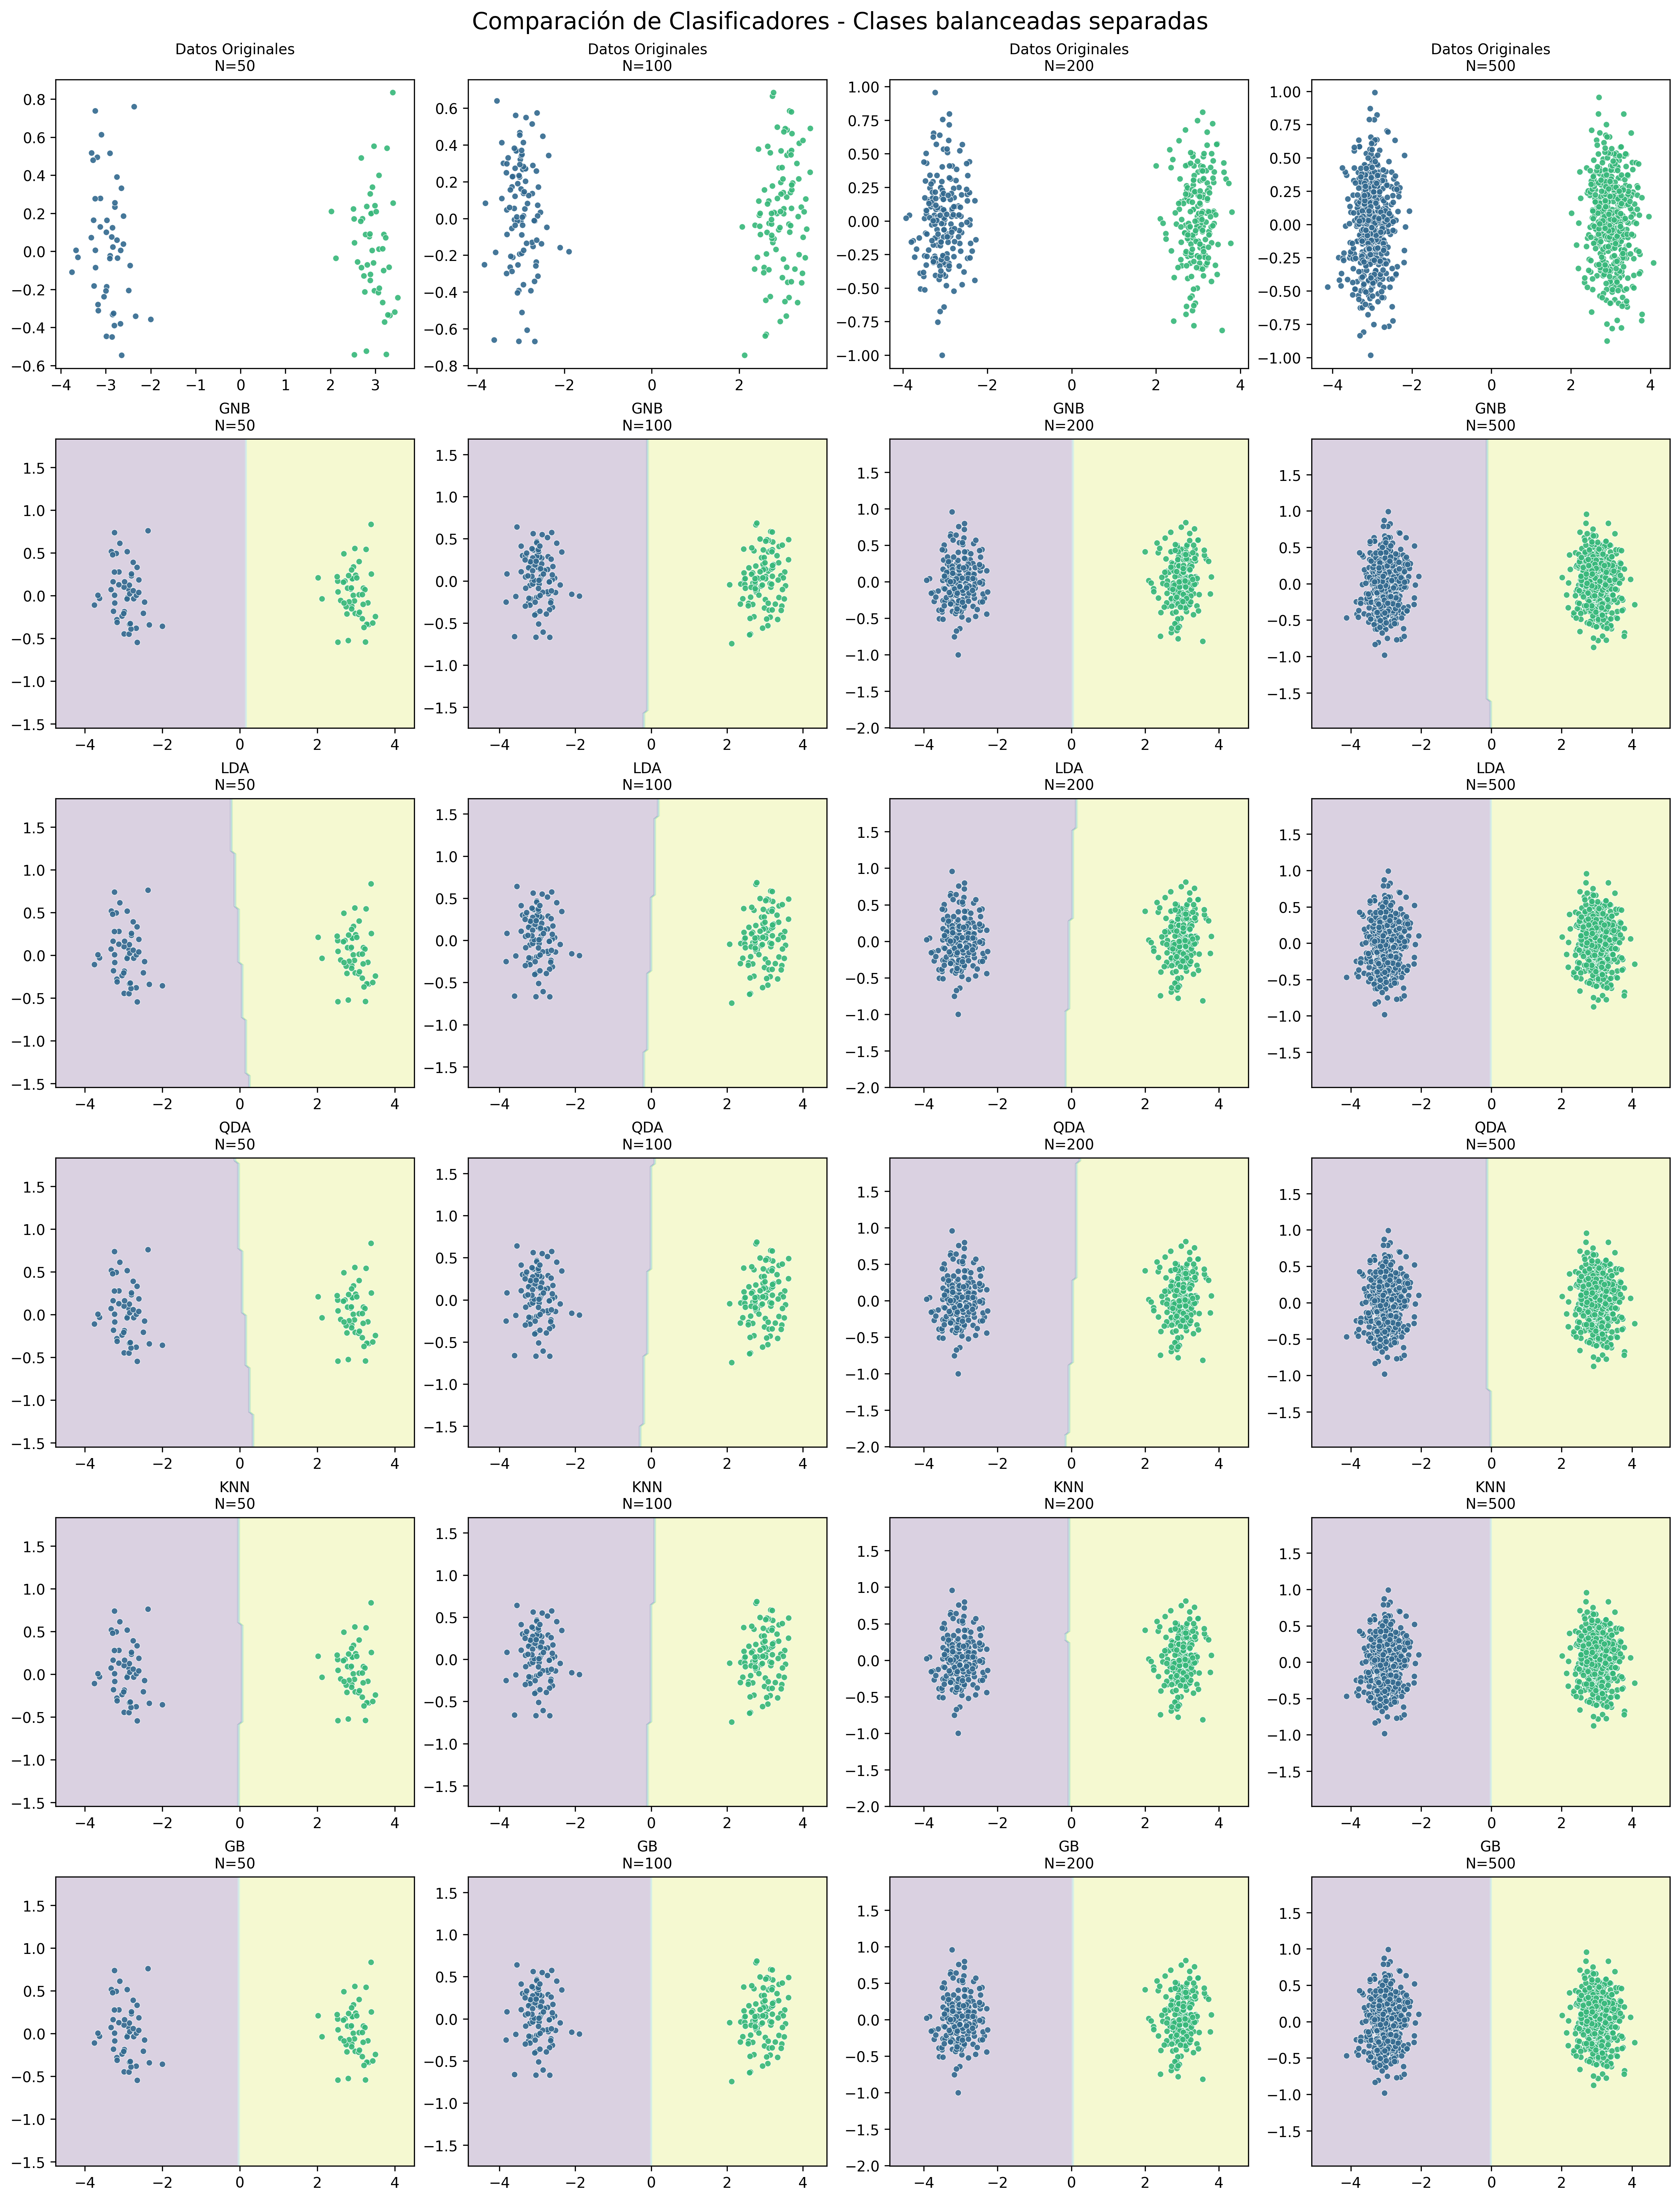
\includegraphics[height=0.4\textheight]{./Parte 2/figures/classifier_comparison_balanced_separated_classes.png}
    \caption{Comportamiento de clasificadores con datos balanceados y clases separadas.}    
    \label{fig:classifier-comparison-balanced-separated-classes}
\end{figure}

% Argumentar lo de arriba
\newpage

\subsubsection*{Clases sobrepuestas}

Los clasificadores con las clases sobrepuestas se comportaron como la Figura
\ref{fig:classifier-comparison-balanced-joined-classes}.

\begin{figure}[!ht]
    \centering
    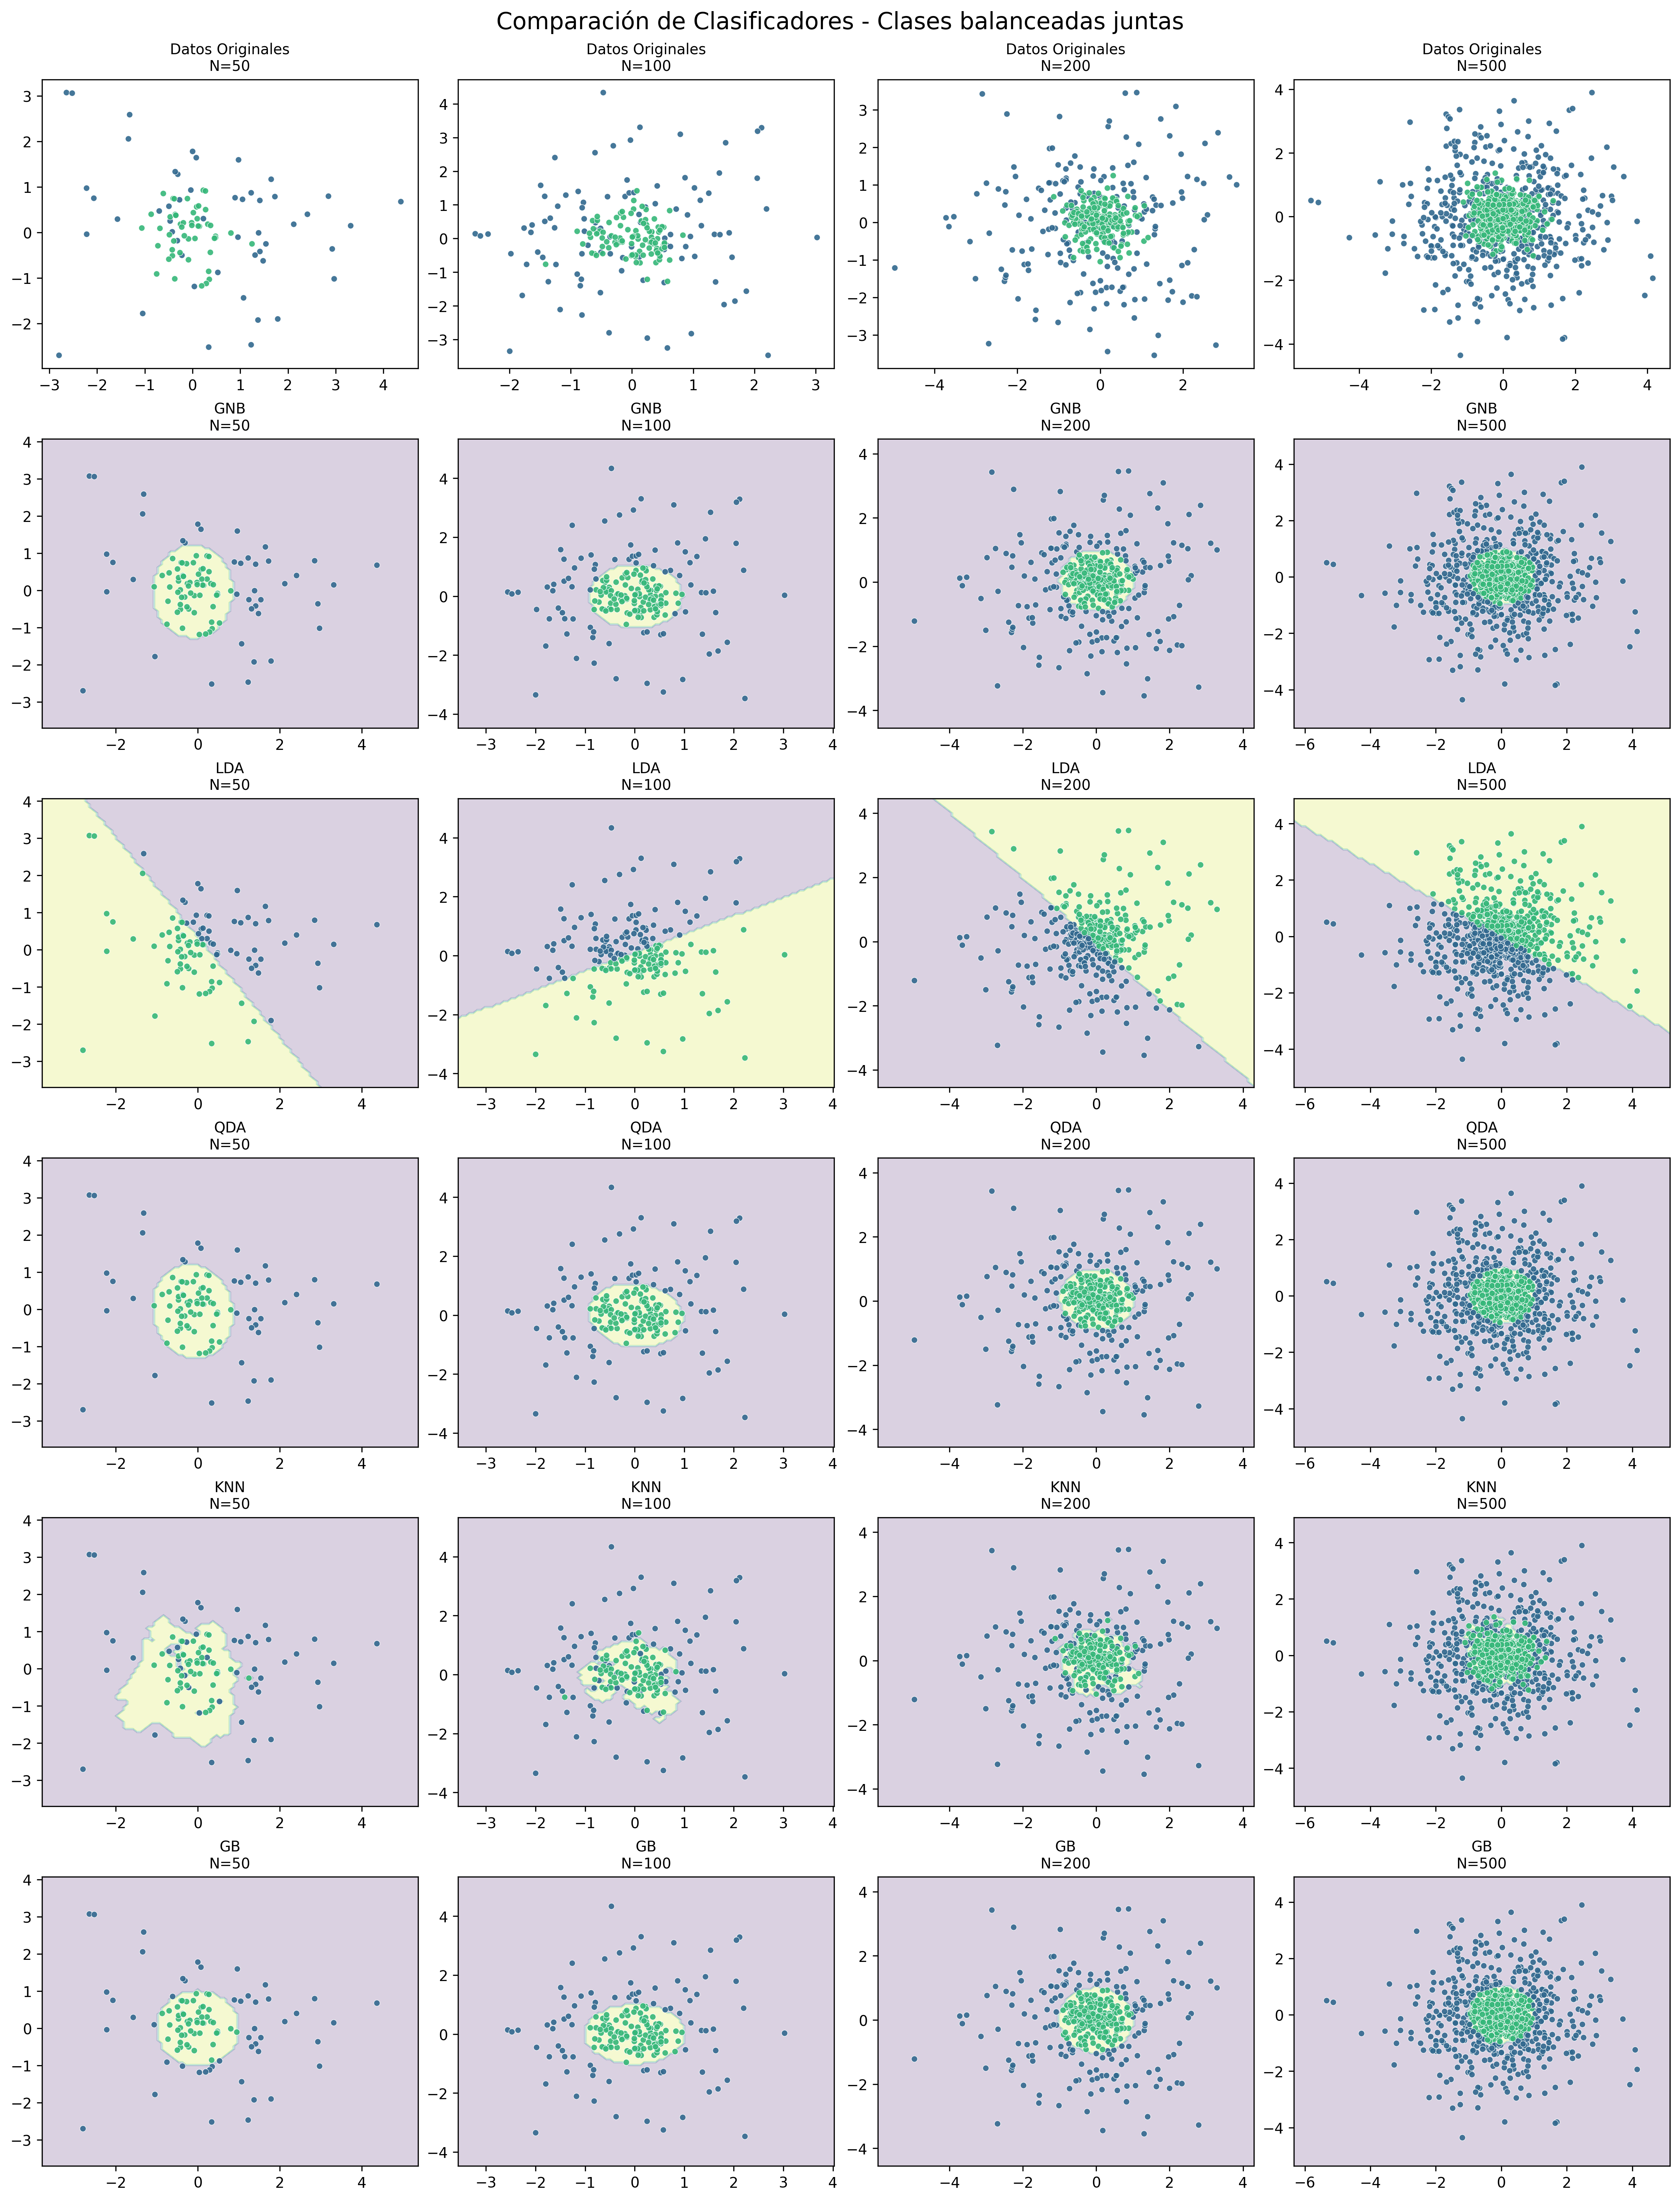
\includegraphics[height=0.4\textheight]{./Parte 2/figures/classifier_comparison_balanced_joined_classes.png}
    \caption{Comportamiento de clasificadores con datos balanceados y clases separadas.}    
    \label{fig:classifier-comparison-balanced-joined-classes}
\end{figure}

% Argumentar lo de arriba
\newpage

\subsubsection*{Datos Balanceados}

A partir de este punto, las simulaciones se realizan con las medias
$\mu_0=(-1,0)$ y $\mu_1=(0, 1)$ para sus respectivas clases, a menos que se
indique lo contrario.

Para datos generados con la misma covarianza se observan las siguientes
comparaciones en la Figura \ref{fig:classifier-comparison-balanced-same-cov}

\begin{figure}[!ht]
    \centering
    \includegraphics[height=0.4\textheight]{./Parte 2/figures/classifier_comparison_balanced_same_cov.png}
    \caption{Comportamiento de clasificadores con datos balanceados y covarianzas iguales.}    
    \label{fig:classifier-comparison-balanced-same-cov}
\end{figure}

\newpage

Para datos generados con distintas covarianzas se observan las siguientes
comparaciones en la Figura \ref{fig:classifier-comparison-balanced-distinct-cov}

\begin{figure}[!ht]
    \centering
    \includegraphics[height=0.4\textheight]{./Parte 2/figures/classifier_comparison_balanced_distinct_cov.png}
    \caption{Comportamiento de clasificadores con datos balanceados y covarianzas distintas.}    
    \label{fig:classifier-comparison-balanced-distinct-cov}
\end{figure}

% Argumentar lo de arriba
\newpage

\subsubsection*{Datos Desbalanceados}

Para datos generados con la misma covarianza se observan las siguientes
comparaciones en la Figura \ref{fig:classifier-comparison-unbalanced-same-cov}

\begin{figure}[!ht]
    \centering
    \includegraphics[height=0.4\textheight]{./Parte 2/figures/classifier_comparison_unbalanced_same_cov.png}
    \caption{Comportamiento de clasificadores con datos desbalanceados y covarianzas iguales.}    
    \label{fig:classifier-comparison-unbalanced-same-cov}
\end{figure}

\newpage

Para datos generados con distintas covarianzas se observan las siguientes
comparaciones en la Figura \ref{fig:classifier-comparison-unbalanced-distinct-cov}

\begin{figure}[!ht]
    \centering
    \includegraphics[height=0.4\textheight]{./Parte 2/figures/classifier_comparison_unbalanced_distinct_cov.png}
    \caption{Comportamiento de clasificadores con datos desbalanceados y covarianzas distintas.}    
    \label{fig:classifier-comparison-unbalanced-distinct-cov}
\end{figure}

% Argumentar lo de arriba
\newpage

\subsubsection*{Variando $K$ en \textit{K-NN}}

Ademas, en el algoritmo de \textit{k-NN} se puede variar el valor de $k$ para
obtener diferentes resultados. De mismo modo, consideraremos clases balanceadas
y clases desvalanceadas, ambas con las mismas covarianzas.

Para clases balanceadas se observan las siguientes comparaciones en la Figura
\ref{fig:knn-study-balanced}.

\begin{figure}[!ht]
    \centering
    \includegraphics[height=0.4\textheight]{./Parte 2/figures/knn_study_balanced.png}
    \caption{Comportamiento de clasificadores con datos desbalanceados y covarianzas distintas.}    
    \label{fig:knn-study-balanced}
\end{figure}

\newpage

Para clases desbalanceadas se observan las siguientes comparaciones en la Figura
\ref{fig:knn-study-unbalanced}.

\begin{figure}[!ht]
    \centering
    \includegraphics[height=0.4\textheight]{./Parte 2/figures/knn_study_unbalanced.png}
    \caption{Comportamiento de clasificadores con datos desbalanceados y covarianzas distintas.}    
    \label{fig:knn-study-unbalanced}
\end{figure}

% Argumentar lo de arriba
\newpage

\subsection*{Analisis de riesgo}


\begin{figure}[!ht]
    \centering
    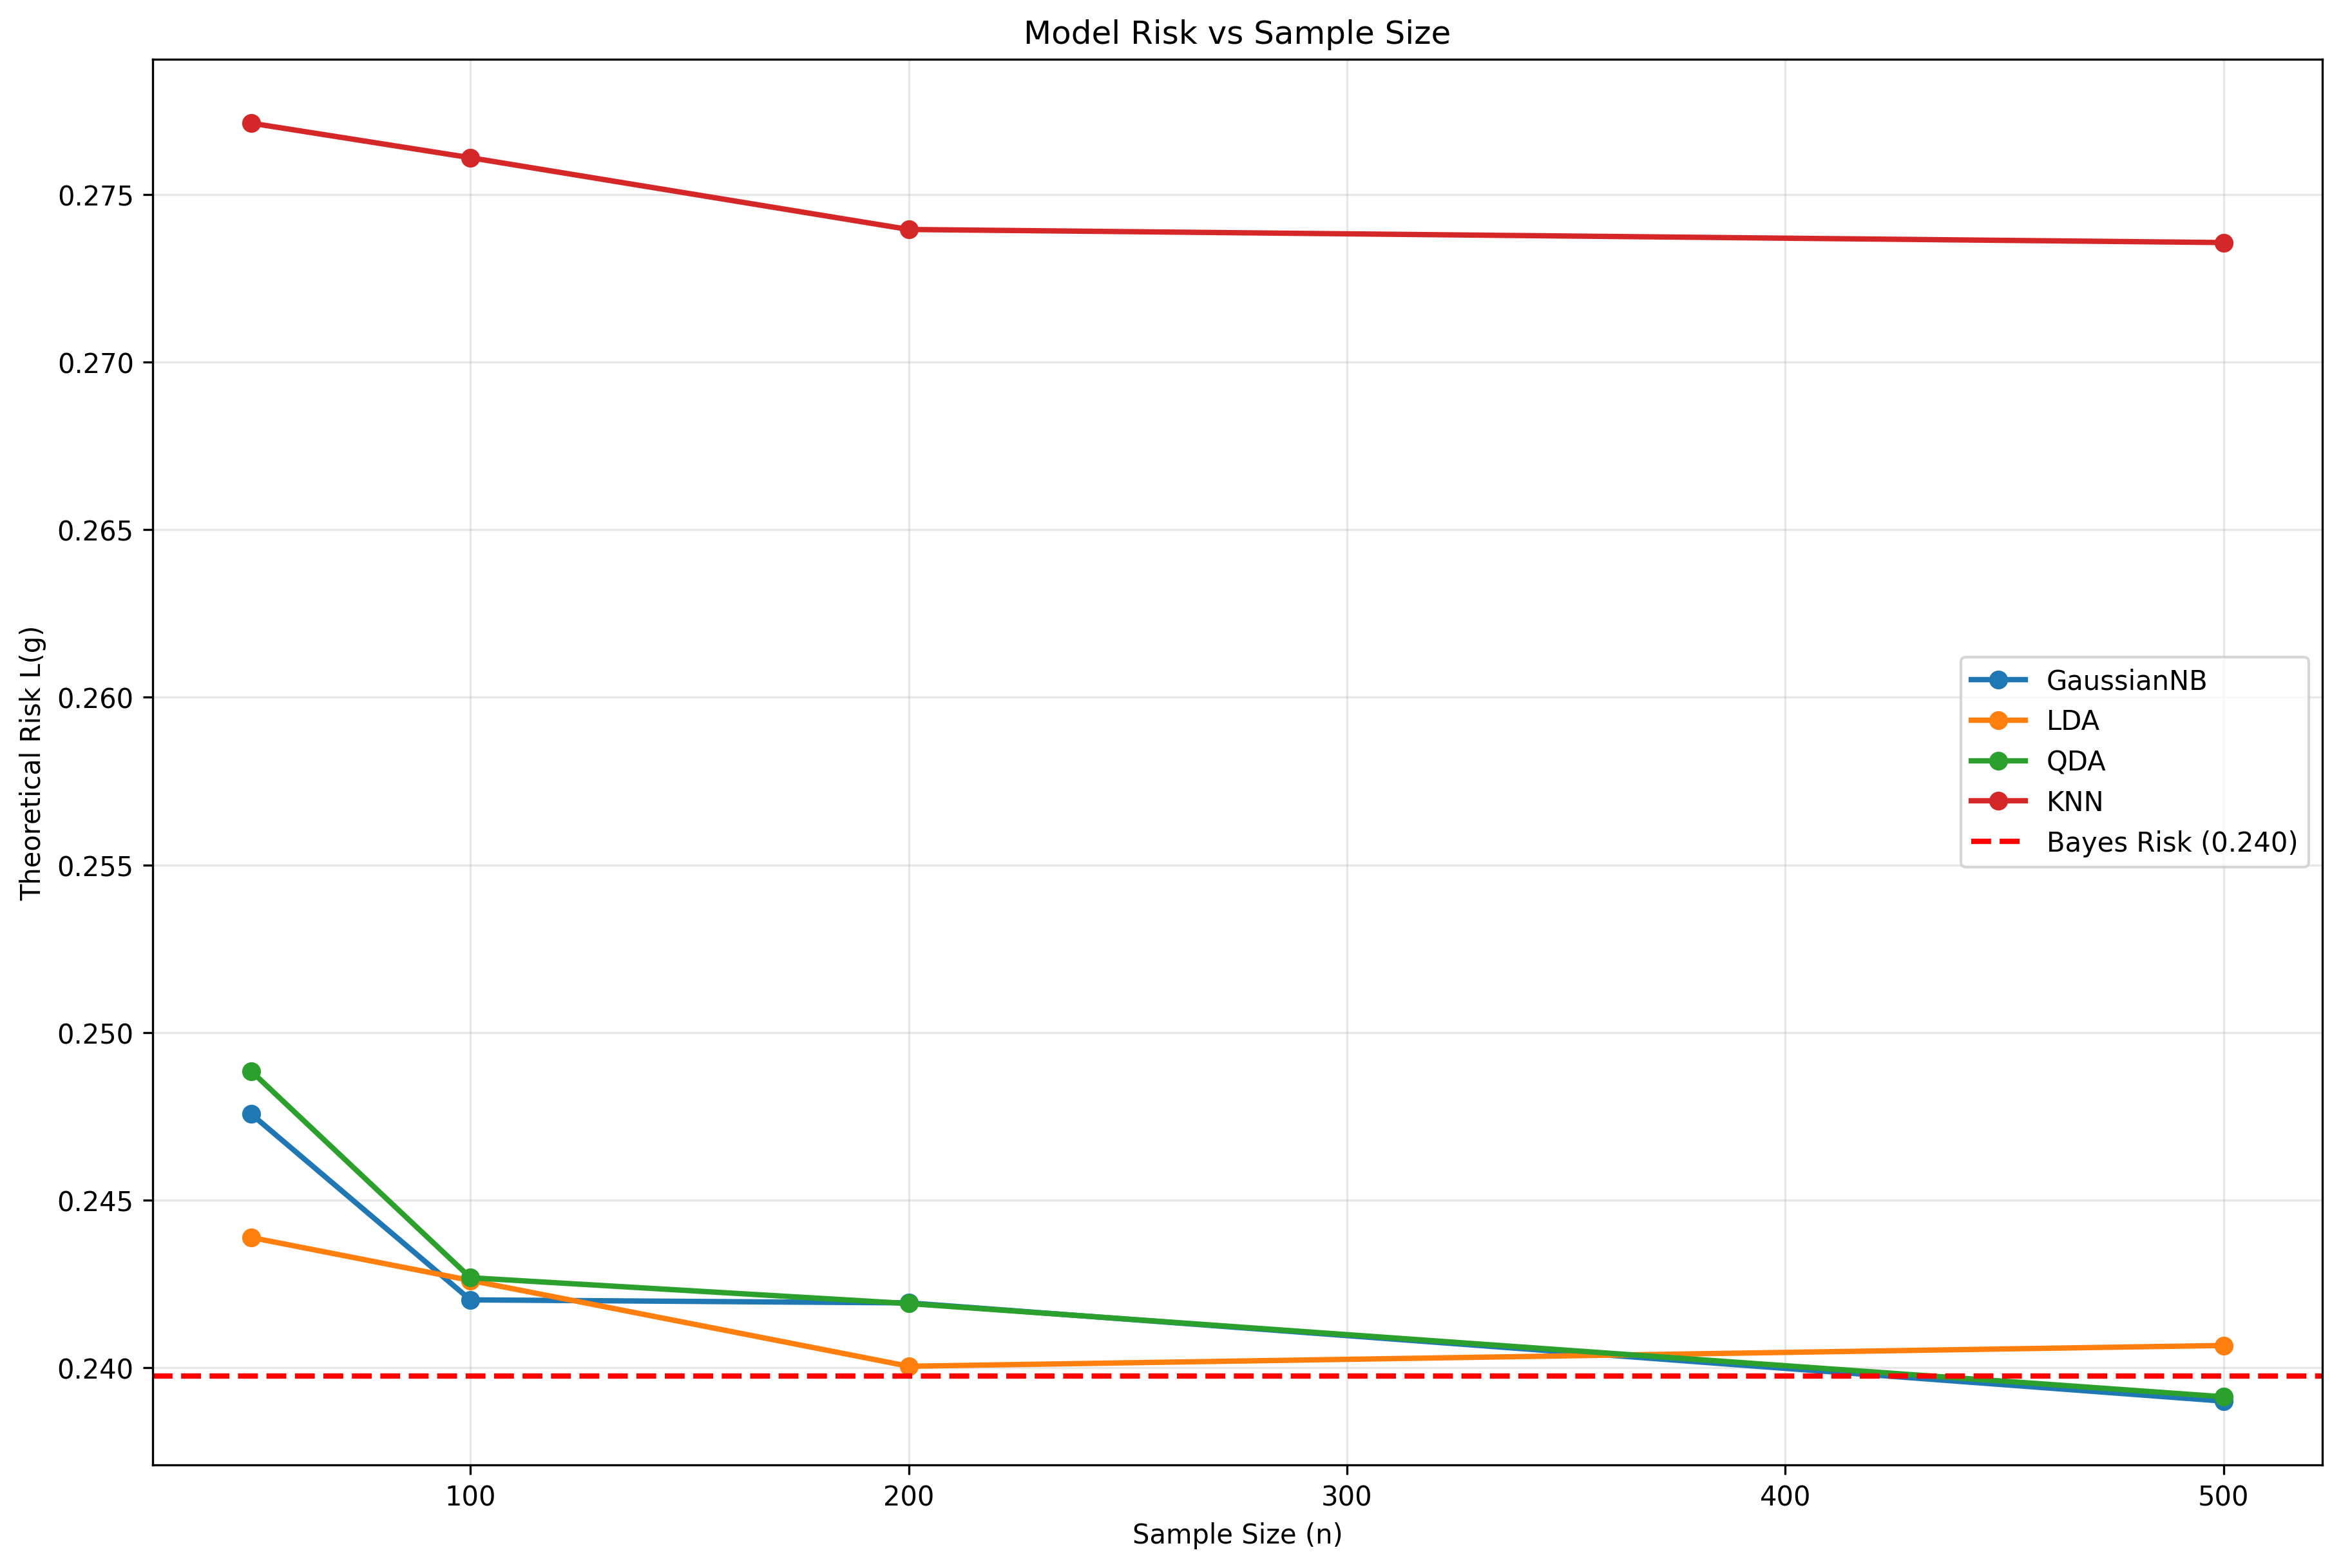
\includegraphics[width=0.8\textwidth]{./Parte 2/figures/risk_vs_samplesize.png}
    \caption{}
    \label{fig:risk-vs-samplesize}
\end{figure}

\newpage

\begin{figure}[!ht]
    \centering
    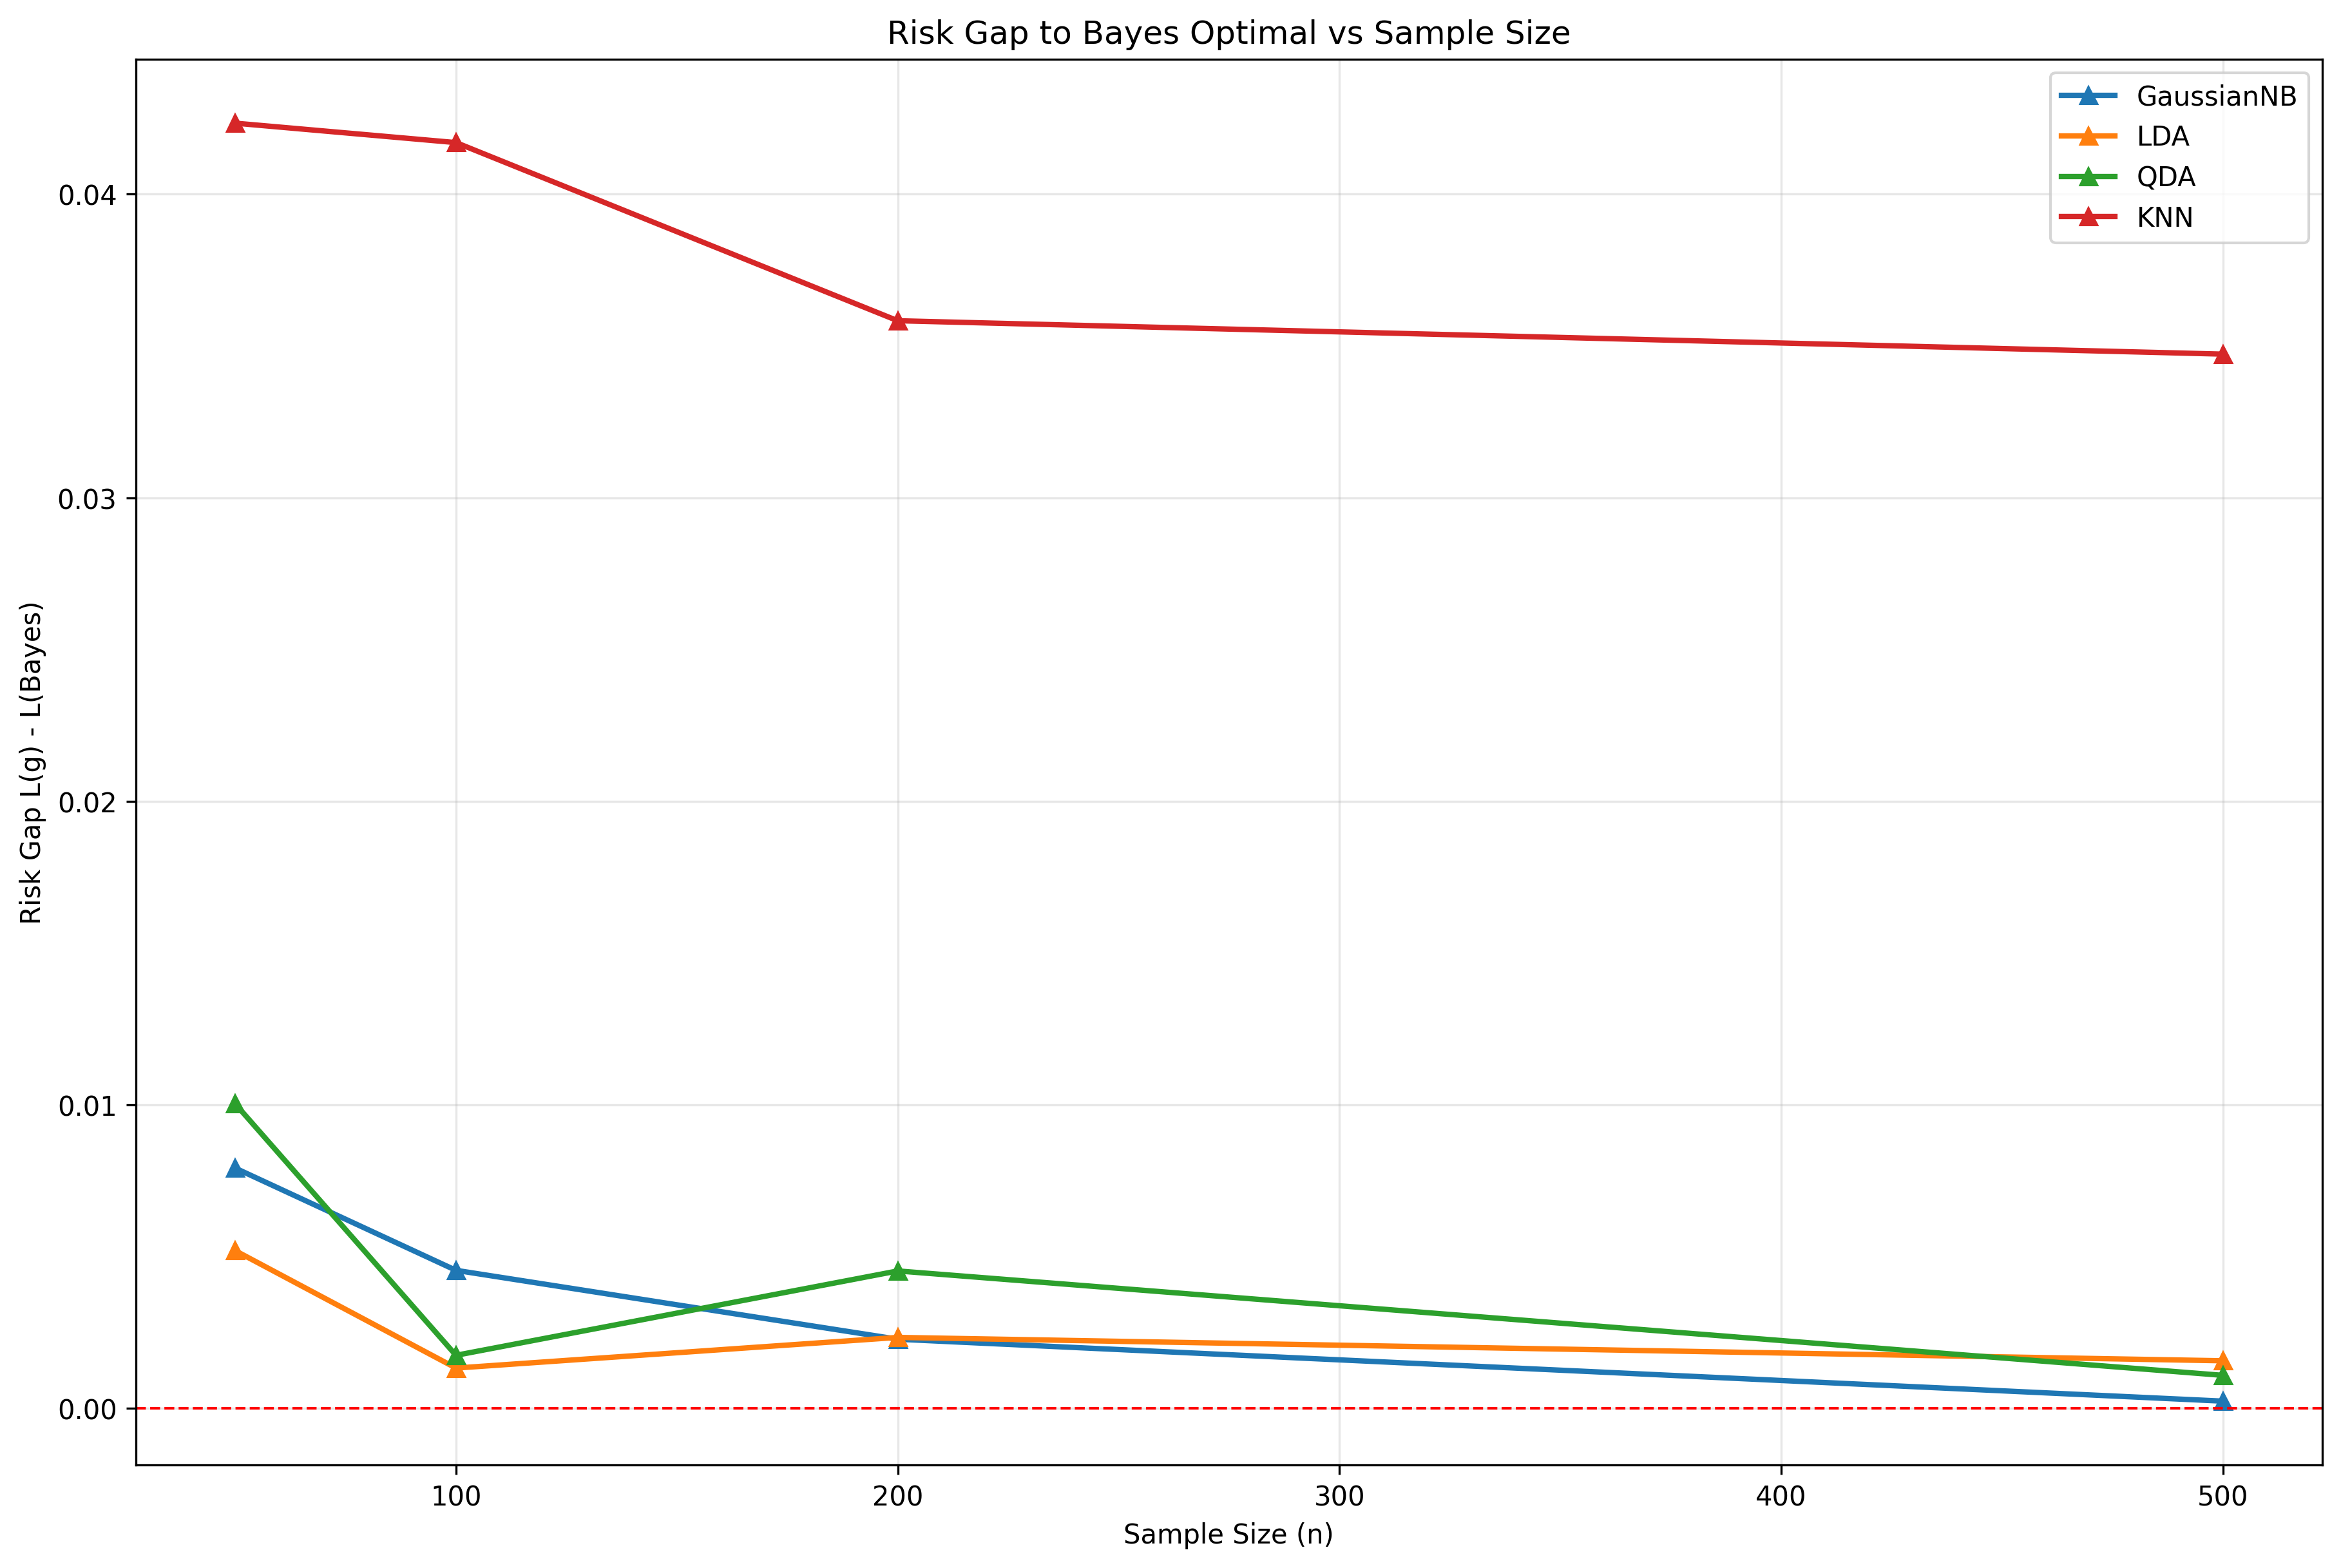
\includegraphics[width=0.4\textwidth]{./Parte 2/figures/risk_gaps.png}
    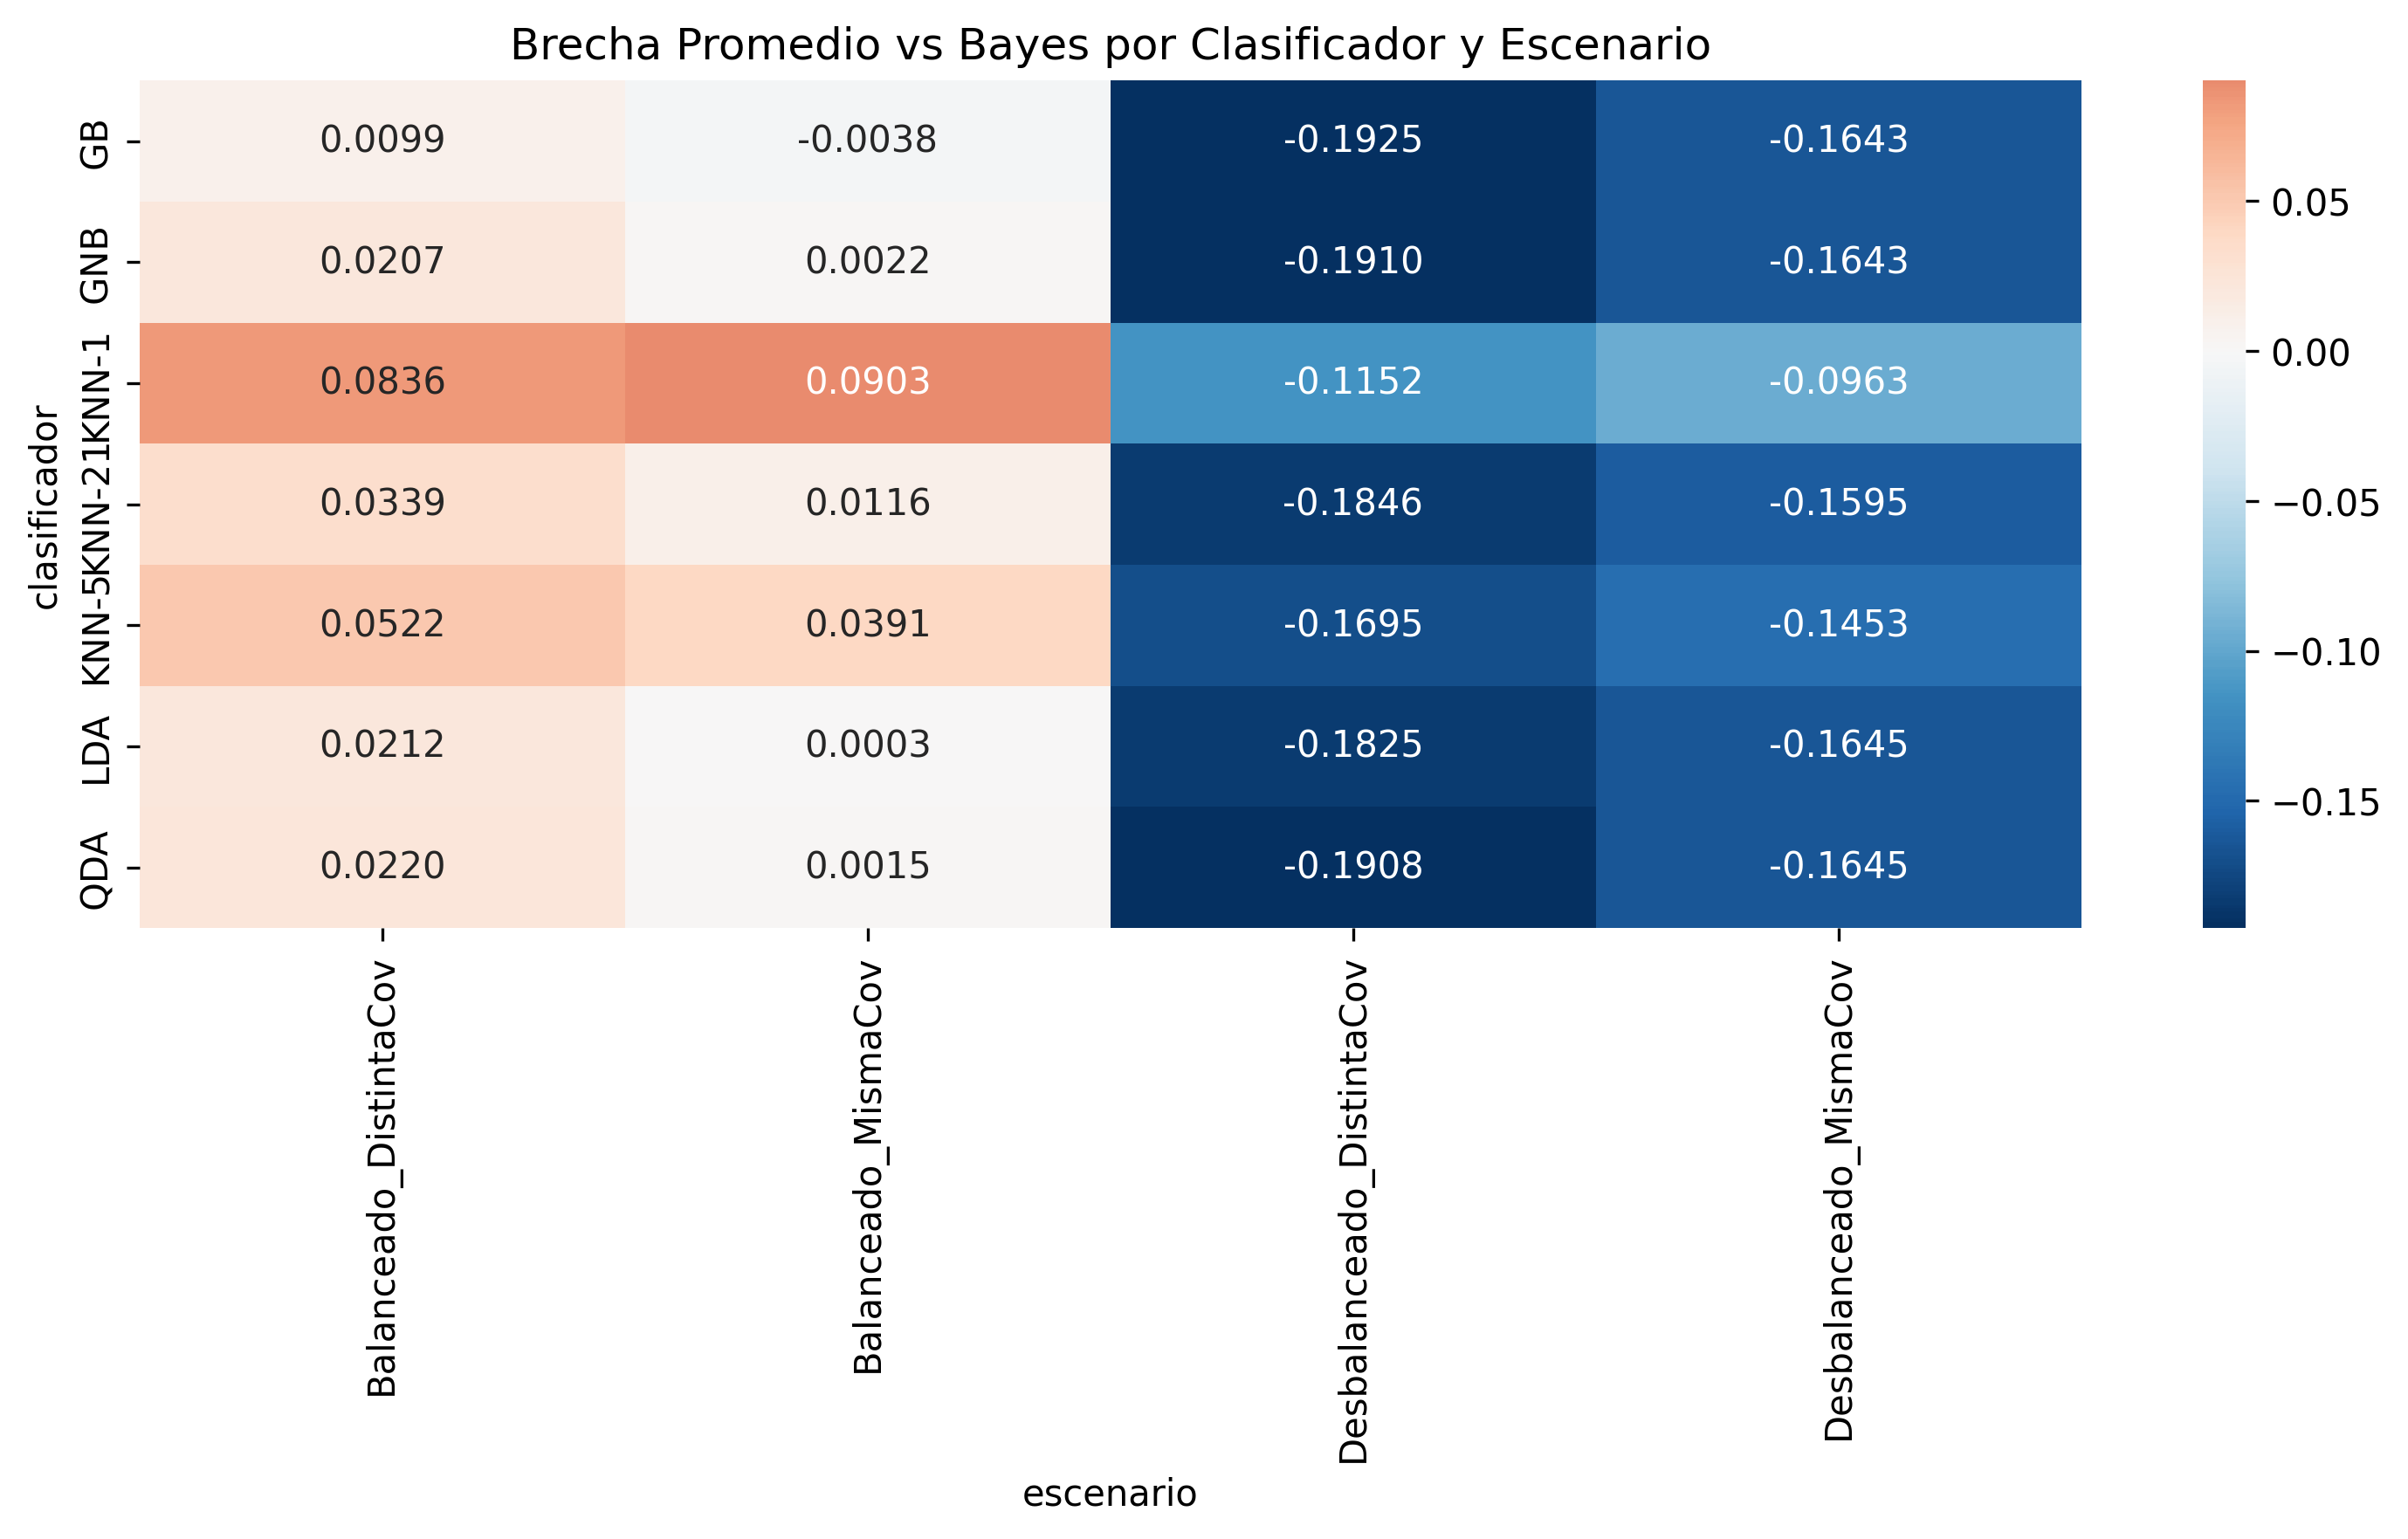
\includegraphics[width=0.4\textwidth]{./Parte 2/figures/risk_gap_heatmap.png}
    \caption{Risk Gaps $L(g) - L(Bayes)$}
    \label{fig:risk-gaps-images}
\end{figure}

\begin{figure}[!ht]
    \centering
    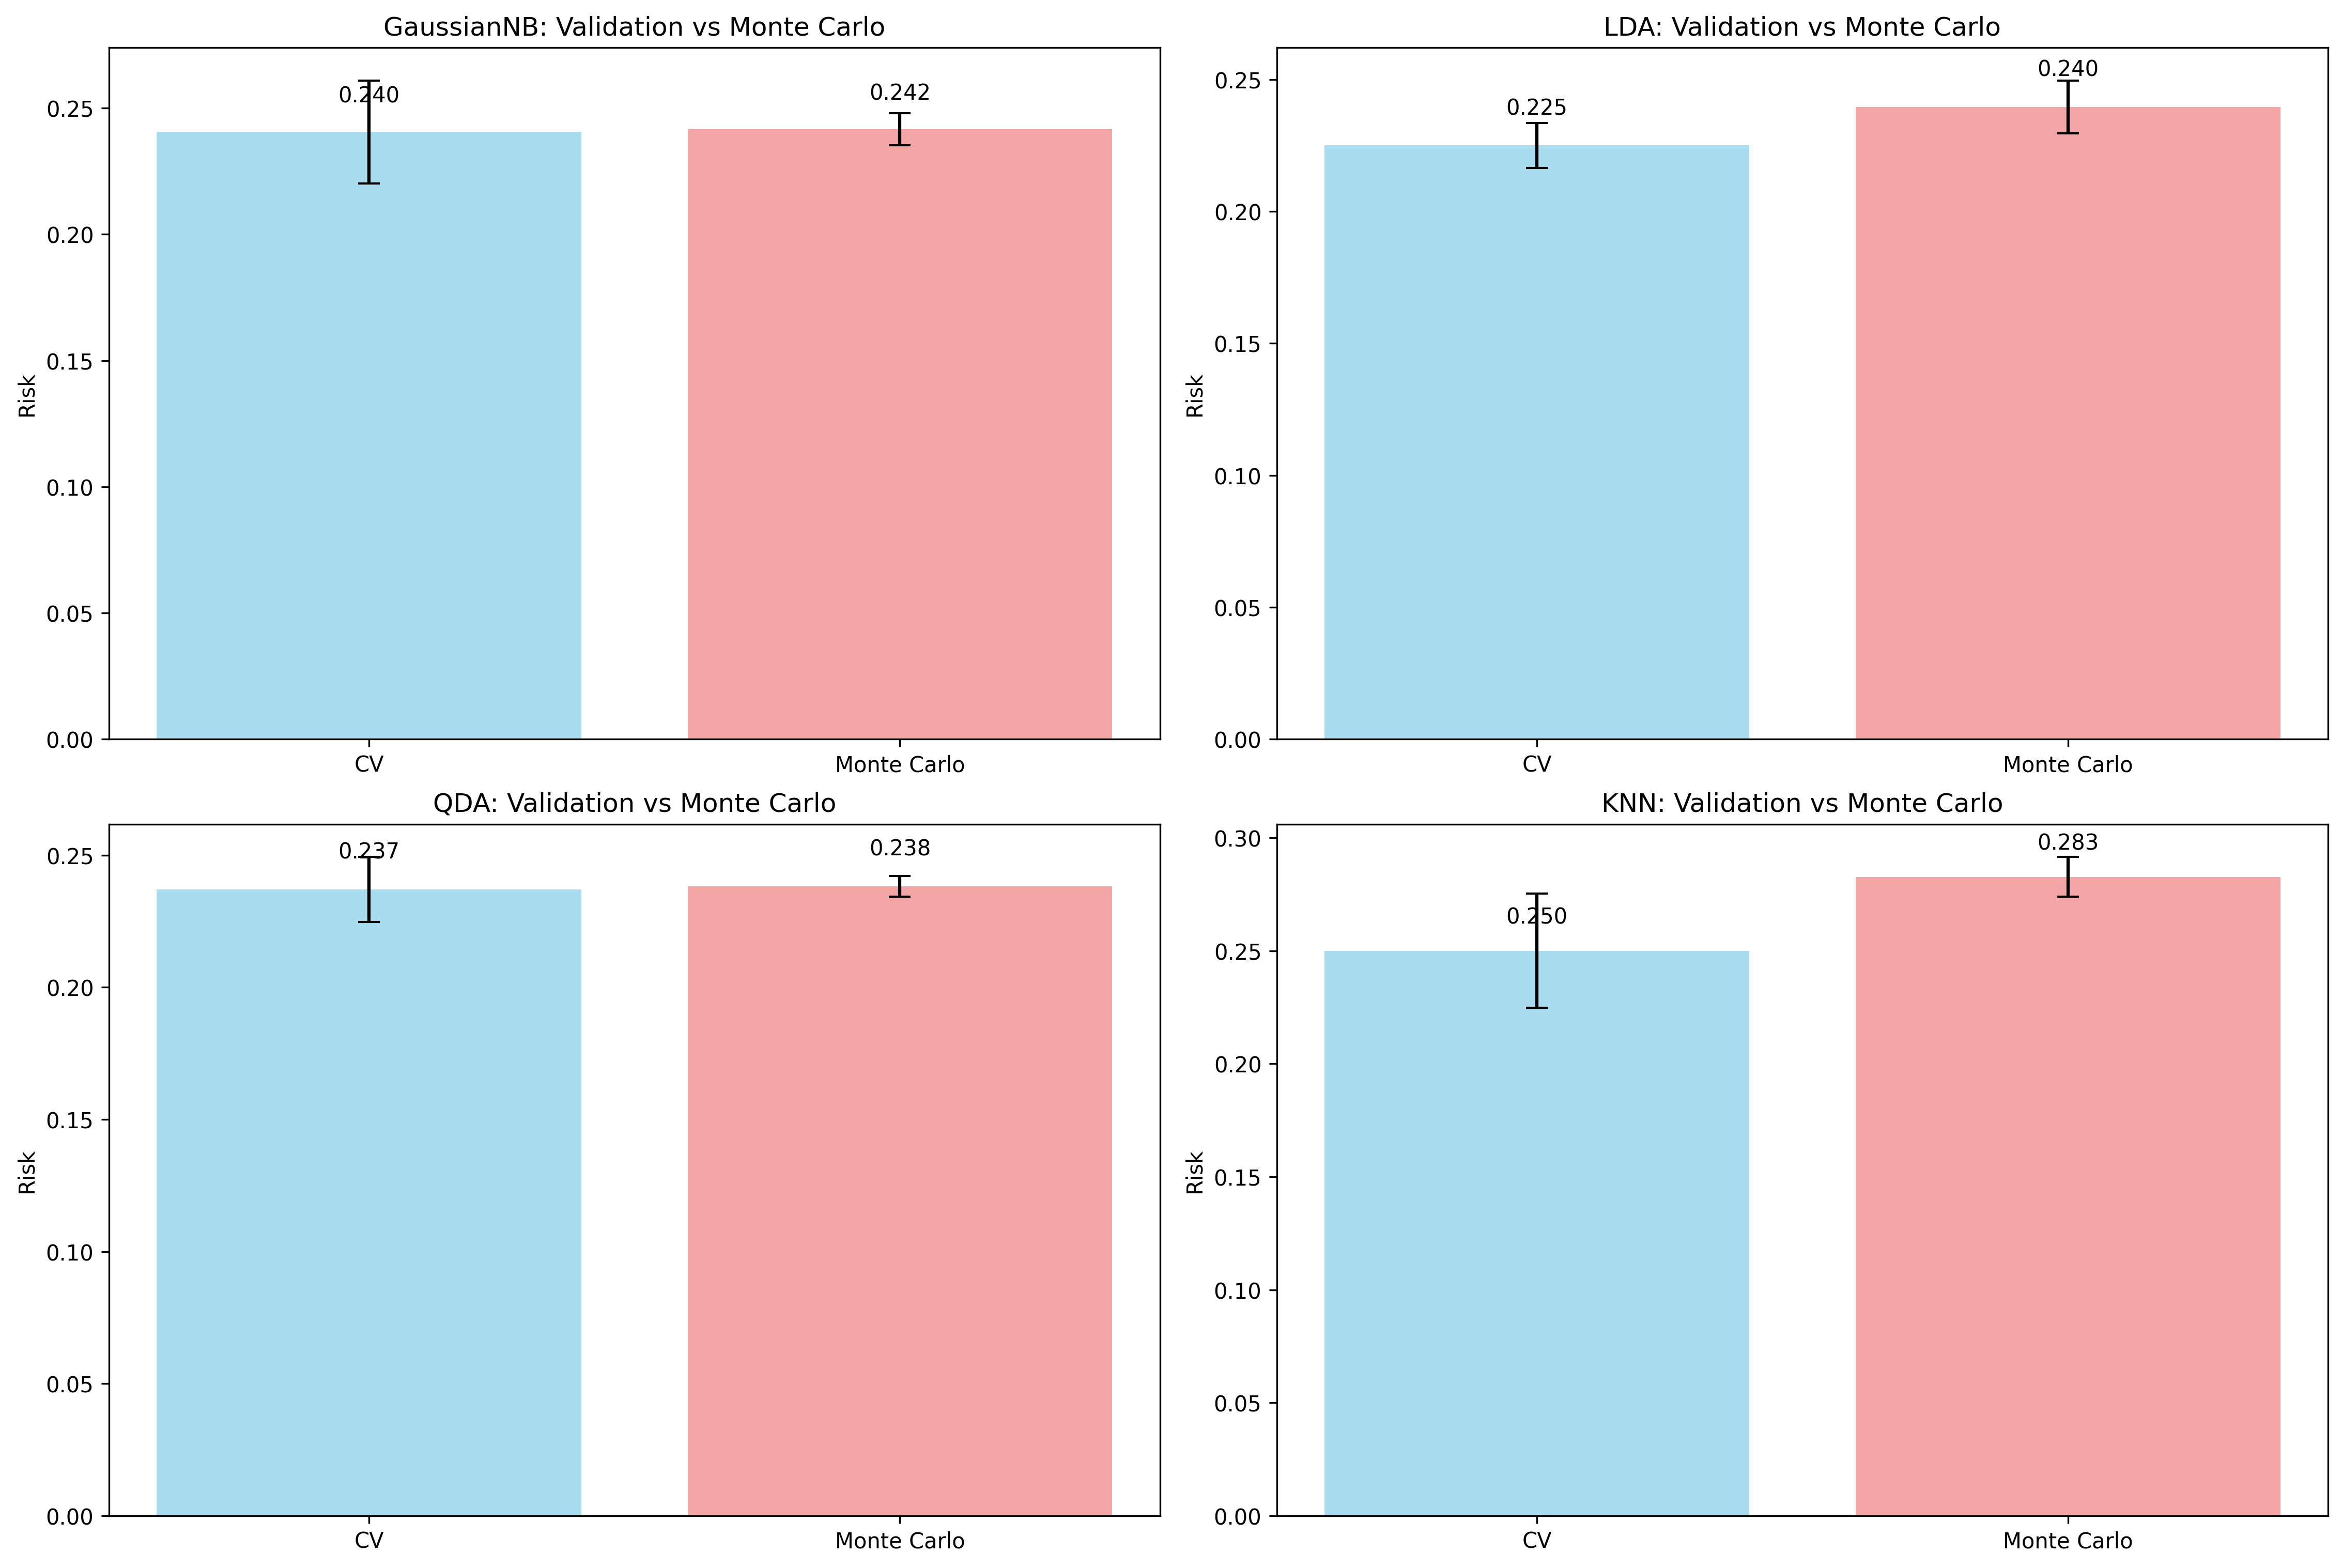
\includegraphics[width=0.8\textwidth]{./Parte 2/figures/validation_comparison.png}
    \caption{Monte Carlo vs Cross Validation}
    \label{fig:mc-vs-cv}
\end{figure}


% ================================================================================
% TABLA RESUMEN: Riesgos Promedio y Desviaciones Estándar
% ================================================================================
% Modelo       Riesgo Promedio Desv Estándar   Gap vs Bayes
% --------------------------------------------------------------------------------
% GaussianNB   0.2435          0.0108          0.0037
% LDA          0.2423          0.0103          0.0026
% QDA          0.2441          0.0098          0.0043
% KNN          0.2784          0.0161          0.0386
% --------------------------------------------------------------------------------
% BAYES        0.2398          -               0
% ================================================================================

% ============================================================
% COMPARACIÓN: Cross-Validation vs Monte Carlo
% ============================================================
% Modelo       CV Risk    CV Std     MC Risk    MC Std
% ------------------------------------------------------------
% GaussianNB   0.2460     0.0155     0.2359     0.0049
% LDA          0.2310     0.0284     0.2430     0.0108
% QDA          0.2350     0.0173     0.2351     0.0091
% KNN          0.2920     0.0410     0.2774     0.0128
% ============================================================

\end{document}